\section{Deformable Simplicial Complexes}
\label{sec:dsc}

This section will describe the DSC framework and the theory it's built upon.

\subsection{Simplices}

A simplex (simplices in plural) is a generalisation of the notion of a triangle
to an arbitrary number of dimensions. The triangle is as such a 2-simplex and it
is the convex hull of its three vertices. More formally we can state a
$n-$dimensional simplex (a $n-$simplex) as the convex hull of its $n+1$
vertices, furthermore a $n$-simplex contains $n+1$ ($n-1$)-simplices, the
exception being the 0-simplex which is the lowest dimensional simplex.

\begin{figure}[h!]
        %====================
        % TODO: Fix this figures, its not pretty :(
        %====================
        \centering
        \begin{subfigure}[b]{0.1\textwidth}
                
\includegraphics[width=\textwidth]{img/0simplex.png}
                \caption{A 0-simplex. (point)}
                \label{fig:0simplex}
        \end{subfigure}%
        \qquad
        \begin{subfigure}[b]{0.2\textwidth}
                
\includegraphics[width=\textwidth]{img/1simplex.png}
                \caption{A 1-simplex. (line)}
                \label{fig:1simplex}
        \end{subfigure}
        ~
        \begin{subfigure}[b]{0.3\textwidth}
                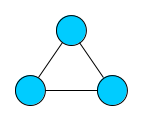
\includegraphics[width=\textwidth]{img/2simplex.png}
                \caption{A 2-simplex. (triangle)}
                \label{fig:2simplex}
        \end{subfigure}%
        ~
        \begin{subfigure}[b]{0.2\textwidth}
                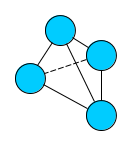
\includegraphics[width=\textwidth]{img/3simplex.png}
                \caption{A 3-simplex. (tetrahedron)}
                \label{fig:3simplex}
        \end{subfigure}

        \caption{The four different simplices that are drawable in three dimensions.
                 The 0- and 1-simplex is technically not drawable, but are shown
                 here for clarification.}
        \label{fig:simplices}
\end{figure}

Figure \ref{fig:simplices} illustrate the four simplest simplices:
\begin{itemize}
  \item \textit{0-simplex:} This is a point in a 0-dimensional universe. When
    pulled into a multidimensional universe, it will usually be represented as a
    vertex.

  \item \textit{1-simplex:} This simplex is seen as a straight line with no
    other properties than length. It contains two 0-simplices.

  \item \textit{2-simplex:} The 2-simplex is a triangle, it exists as a
    2-dimensional figure with no "thickness" it is the lowest dimensional
    simplex to have a surface. It contains three 1-simplices.

  \item \textit{3-simplex:} This simplex is called a tetrahedron, it is the
    lowest dimensional simplex to have a volume and not just a surface. It
    contains four 2-simplices.
\end{itemize}



% During this project the most Important simplex is the 3-simplex because I will
% be working with a 3-dimensional mesh, but it is relevant to explain that
% simplex can have an arbitrary number of dimensions and that all simplices
% actually consist of simplices of a lower dimension.

Further definitions on simplices and sets of simplices can be made.
The dimension of a set of simplices $\Sigma$ is the maximum dimension of any
simplex in it. This is formalized as
\[
    \text{dim}(\Sigma) = \text{max}\{\text{dim}(\sigma) | \sigma \in \Sigma \}.
\]
We also define the $k$-subset as a set of all $k$-simplices in $\Sigma$ as
\[
    \text{filter}_k = \{\sigma_i \in \Sigma | \text{dim}(\sigma_i) = k\}.
\]

\subsection{Simplicial Complexes}
Simplicial complexes are groups of simplices that are grouped together to yield
a more complex structure. In order for a group of simplices $\Sigma$ to form a
simplicial complex it will need to satisfy two conditions:
\begin{enumerate*}
    \item $\Sigma$ is closed, such that for any simplex $\sigma \in
          \Sigma$ all the faces of $\sigma$ are in $\Sigma$.

    \item The intersection of any two simplices $\sigma_i \cap
          \sigma_j$ for $\sigma_i,\sigma_j \in \Sigma$ must be a face of both
          $\sigma_i$ and $\sigma_j$.
\end{enumerate*}

Figure \ref{fig:scexamples} shows a simplicial complex and a group of
simplices that do not constitute a simplicial complex since they do not satisfy
the above conditions.

\begin{figure}
        \centering
        \begin{subfigure}[b]{0.4\textwidth}
                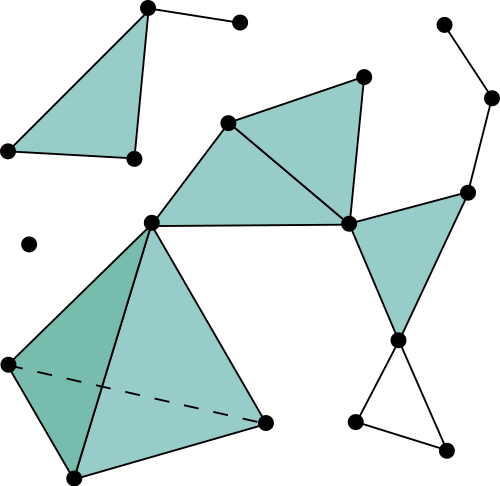
\includegraphics[width=\textwidth]{img/wiki_simplcialcomplex.png}
        \end{subfigure}%
        \qquad
        \begin{subfigure}[b]{0.3\textwidth}
                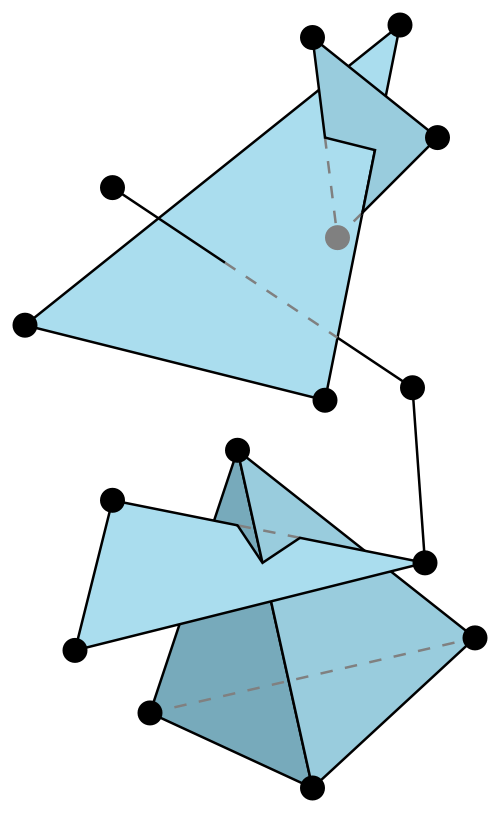
\includegraphics[width=\textwidth]{img/wiki_nonsimplicialcomplex.png}
        \end{subfigure}

        \caption{A valid simplicial complex(left), and a set of simplices
                 that do not qualify as a simplicial complex (right.) Source:
                 Wikipedia.org \cite{wikisc}}
        \label{fig:scexamples}
\end{figure}

%Reinsert this if it is needed for later understanding.
%For any Simplicial complex $K'$ that is a subset of another simplicial complex
%$K' \subset K$ is called a subcomplex of $K$.

In order to later work with a simplicial complex, it is beneficial to
define a number of topological relations for the simplices in a complex. For a
$n-$dimensional simplex $\sigma^n$ in a simplicial complex $K$ we define:
\begin{itemize}
    \item \textit{Boundary}: For $p > q$ the boundary relation is the set of
         $q$-faces of $\sigma^p$ defined as
         \[
            B_ {p,q}(\sigma^p) = \text{filter}_q\{\sigma \in K | \text{vert}(\sigma) \subset \text{vert}(\sigma^p)\}.
         \]

    \item \textit{Coboundary}: For $p < q$ the Coboundary relation is the set of
         all $q$-simplices that have $\sigma^p$ as a face, defined as
         \[
            C_ {p,q}(\sigma^p) = \text{filter}_q \{\sigma \in K | \text{vert}(\sigma^p) \in \text{vert}(\sigma)\}.
         \]
    % Reinsert if needed later
    %\item[Adjecency] for $p >0$ the adjecency relation is a set of all
    %     $p$-simplices which share a $p-1$-face with $\sigma^p$:
    %     \[
    %        A_p(\sigma^p) = filter_p\{\sigma \in K : |vert(\sigma^p) \cap vert(\sigma)|=p\}
    %     \]
\end{itemize}

We will now use these to define the \emph{star}, \emph{link} and \emph{closure}
of a simplex $\sigma$.

The star of a simplex $\sigma$ is the set of all simplices in $K$ which have
$\sigma$ as a face (for illustration see Figure \ref{fig:star})
\[
  \text{star}(\sigma^p) = \{ \sigma \in K | \text{vert}(\sigma^p) \in \text{vert}(\sigma) \} = \bigcup_{q=p+1}^{n}C_{p,q}(\sigma^p).
\]
\graphicc{0.6}{img/wiki_star.png}{The star(green) of one simplex(yellow).
Source: Wikipedia.org \cite{wikisc}}{fig:star}

We also define the closure of a simplex $\sigma^p \in K$ as the set (for
illustration see Figure \ref{fig:closure})
\[
  \text{closure}(\sigma^p) = \bigcup_{q=0}^{p}B_ {p,q}(\sigma^p).
\]
\graphicc{0.6}{img/wiki_closure.png}{The closure(green) of two simplices
(yellow). Source: Wikipedia.org \cite{wikisc}}{fig:closure}

Finally we define the link of a simplex (for illustration see Figure \ref{fig:link}) as
\[
  \text{link}(\sigma) = \text{closure}(\text{star}(\sigma)-\text{star}(\text{closure}(\sigma))).
\]
\graphicc{0.6}{img/wiki_link.png}{The link(green) of one simplix(yellow).
Source: Wikipedia.org \cite{wikisc}}{fig:link}

Both the star- and closure-operation can be defined as the union of the results
of running the operation on each subsimplex formally expressed as
\[
  \text{star}(\Sigma) = \bigcup_{\sigma_i \in \Sigma} \text{star}(\sigma_i)
\]
and
\[
  \text{closure}(\Sigma) = \bigcup_{\sigma_i \in \Sigma} \text{closure}(\sigma_i).
\]


\subsection{Deformable Simplicial Complexes}
DSC is a framework for 3D tetrahedral meshes which supplies a set of operations
and promises to always optimize its mesh. DSC works inside a ``computational
domain'', this domain further contains a number of sub-domains that are either
\textit{inside} (a mesh in the world) or \textit{outside} (the volume around the
mesh.) DSCs domain is a tetrahedral mesh (a simplicial complex) that satisfies
the two criteria
\begin{itemize}
  \item \textit{Simplicial Complex Criterion:} The intersection between two
        simplices must be either empty or their common face. For a tetrahedron,
        that is the common face, edge or vertex.
  \item \textit{Conform To Interface:} The interface of a DSC is a set of
        boundary vertices/edges/faces between simplices that are marked as being
        either inside or outside.
\end{itemize}

This allows the DSC framework to contain several meshes in its domain (several
\textit{inside} sub-domains.) and let them merge together into a single domain.
Figure \ref{fig:meshmelt} shows an example of two domains melting together to
form a single domain. The example is drawn in 2 dimensions for clarity.

\graphicc{1.0}{img/mesh_melt.png}{Two domains melting together to form a single
domain. Blue simplices are inside, grey are outside.
Source: Misztal\cite{DSC10}.}{fig:meshmelt}

Part of the merging process is moving the vertices. On p. 50 of \cite{DSC10}
\texttt{Algorithm 4} and \texttt{Algorithm 5} describes how DSC moves vertices
around. When moving a vertex, DSC will calculate if the move will cause the
vertex to intersect with any simplex that is in the \textit{link} of the vertex.
If there is an intersection the vertex will be moved to the intersection, if
there is no intersection, the vertex will be moved the full length. This is
seen on Figure \ref{fig:meshmelt} where a vertex moves into contact with an
edge that is part of its \textit{link}.

One of the benefits of the DSC framework is that it will automatically make
sure that all of its tetrahedrons have a certain quality. DSC ascertain its own
quality by looking at the quality of the worst tetrahedron in the mesh as well
as seven threshold means (p. 34 \cite{DSC10}). A quality mean
$\overline{q}_\theta$ with the threshold $\theta$ is computed as
\[
  \overline{q}_\theta = \frac{1}{\text{No. of tetrahedra in M}}
  \sum_{t \in M}^{}(\text{min}(q(t),\theta)),
\]

where $M$ is the mesh and $q$ is the tetrahedron quality measure. The seven
different thresholds used in DSC are: $sin(1^\circ)$, $sin(5^\circ)$,
$sin(10^\circ)$, $sin(15^\circ)$, $sin(25^\circ)$, $sin(35^\circ)$ and
$sin(45^\circ)$. Using a broader measurement over all the tetrahedra instead of
just going with the quality of the worst tetrahedron yields a better overall
assessment of the mesh, and reflects better if the mesh is being optimized since
the worst tetrahedron may not have been optimized. The mesh optimization loop
of the mesh will terminate if either the worst tetrahedron improves or one of
the thresholds improves by at least $0.0001$.

The mesh improvement algorithm used by DSC is described as \texttt{Algorithm 1}
in pseudocode on p. 55 of \cite{DSC10}. DSC will first run a vertex smoothing
pass and a topological pass on the mesh. After this it will enter a loop that
will not break until it have made three iterations where the mesh have not improved
sufficiently. For each pass it will attempt a vertex smoothing pass, a
topological pass and a thinning pass. The Topological pass is described as
\texttt{Algorithm 2} on the same page, and the thinning pass is described as
\texttt{Algorithm 3} on p. 56 of \cite{DSC10}. The vertex smoothing algorithm
is called \textit{Laplacian Smoothing} \cite{wikils}. It works by adding all
the neighbours of the node we want to smooth, and dividing the resulting vector
by the number of neighbours
\[
  \overline{x_i} = \frac{1}{N}\sum_{j=1}^{N}x_j,
\]
where $\overline{x_i}$ is the new position of the vertex, and $N$ is the number
of vertices addjecent to $x_i$.

The topological pass will try to take each edge and face of all the tetrahedra
and attempt to remove it using its built-in edge removal algorithm and
multi-face re-triangulation.

The thinning pass will go over all the edges in the mesh and attempt to collapse
it. It will first try and collapse its vertex $b$ into the vertex $a$, and
smooth the position of $b$. If this does not work, it will attempt to collapse
$a$ into $b$ and smooth $b$.